\documentclass[journal]{IEEEtran}
\usepackage{amsmath,graphicx,url,subfig,multirow}
\hyphenation{op-tical net-works semi-conduc-tor}

\begin{document}

\title{FDTD Analysis of Radiation from Infinite Current Line with PML Boundary Conditions}
\author{Yushi~Zhou}
\maketitle

\begin{abstract}
This paper presents a finite-difference time-domain (FDTD) analysis of radiation from an infinite harmonic current line, 
with a focus on implementing perfectly matched layer (PML) boundary conditions. The simulation is based on Yee's staggered grid algorithm, 
which provides natural compatibility with Maxwell's equations. We validate our FDTD implementation against analytical solutions 
derived from Hankel functions, demonstrating convergence with decreasing grid sizes. 
A systematic study of PML parameters reveals optimal configurations, achieving reflection coefficients as low as 
$1.53 \times 10^{-2}$ with a polynomial order of 2 and PML thickness of 0.5$\lambda$. 
The method is further applied to analyze wave propagation through conducting sheets with single and double slots, 
effectively demonstrating diffraction phenomena. Results confirm that the FDTD-PML approach provides 
an accurate and efficient means of simulating unbounded electromagnetic wave problems with complex geometries.
\end{abstract}

\begin{IEEEkeywords}
FDTD, PML, Yee grid,  Wave radiation
\end{IEEEkeywords}

\section{Introduction}
The finite-difference time-domain (FDTD) method based on Yee's spatial grid \cite{yee1966numerical} has become a fundamental approach for solving electromagnetic wave problems. 
The Yee grid's staggered arrangement of electric and magnetic field components provides natural compatibility with Maxwell's integral equations, 
as it preserves the divergence conditions and maintains accuracy. 

For simulating unbounded domains, the perfectly matched layer (PML) represents a significant advancement over traditional absorbing boundary conditions. 
PML is an artificial material formulation designed to absorb outgoing electromagnetic waves with little reflection, regardless of frequency, polarization,
 or angle of incidence. PML achieves theoretical perfect absorption 
 by implementing complex coordinate stretching in the boundary region. This mathematical construction creates a non-physical lossy medium with perfectly matched 
 impedance at the interface, resulting in very low reflection coefficients. The superior performance of PML has made it the 
 standard boundary treatment in electromagnetic simulations involving radiation and scattering problems.

This paper examines the radiation characteristics of an infinite harmonic current line using FDTD simulation with PML boundary conditions. 
After validating the FDTD calculation with analytical solution, we introduced a conducting sheet with one or two slots to test the performance of the FDTD-PML method.

\section{Formulation of FDTD-PML Method}
\subsection{FDTD Discretization}
A infinite current line system perserves cylindrical symmetry, thus can be simplified as a 2D problem.
And because the TM (Transverse Magnetic) Mode and TE (Transverse Electric) Mode are decoupled in 2D space, we can focus on the TM mode, 
which only $E_z$ and $H_x$ , $H_y$ are non-zero. 

In a 2D problem, Maxwell's equations can be written as:
\begin{align}
\frac{\partial H_x}{\partial t} &= -\frac{1}{\mu_0}\frac{\partial E_z}{\partial y} \\
\frac{\partial H_y}{\partial t} &= \frac{1}{\mu_0}\frac{\partial E_z}{\partial x} \\
\frac{\partial E_z}{\partial t} &= \frac{1}{\epsilon}\left(\frac{\partial H_y}{\partial x} - \frac{\partial H_x}{\partial y}\right) - \frac{1}{\epsilon} J_z
\end{align}

The Yee grid discretizes Maxwell's equations as \cite{jin2015theory}:

\begin{align}
H_x^{n+\frac{1}{2}}(i,j) &= H_x^{n-\frac{1}{2}}(i,j) - \frac{\Delta t}{\mu_0\Delta x}\left[E_z^n(i,j+\frac{1}{2}) - E_z^n(i,j)\right] \\
H_y^{n+\frac{1}{2}}(i,j) &= H_y^{n-\frac{1}{2}}(i,j) + \frac{\Delta t}{\mu_0\Delta x}\left[E_z^n(i+\frac{1}{2},j) - E_z^n(i,j)\right] \\  
E_z^{n+1}(i,j) &= \frac{1}{\beta(i,j)}\left[\alpha(i,j) E_z^n(i,j) \right. \nonumber \\
&+ \frac{1}{\Delta x}\left(H_y^{n+\frac{1}{2}}(i+\frac{1}{2},j) - H_y^{n+\frac{1}{2}}(i,j)\right) \nonumber \\
&- \frac{1}{\Delta y}\left(H_x^{n+\frac{1}{2}}(i,j+\frac{1}{2}) - H_x^{n+\frac{1}{2}}(i,j)\right) \nonumber \\
&\left. - J_z^{n+1}(i,j)\right]
\end{align}
where $\alpha(i,j)=\frac{\epsilon(i,j)}{\Delta t}-\frac{\sigma(i,j)}{2}$, $\beta(i,j)=\frac{\epsilon(i,j)}{\Delta t}+\frac{\sigma(i,j)}{2}$.

\subsection{PML Boundary Conditions}
The modified time-domain Maxwell’s equations of PML in 2D space are given by:
\begin{align}
\frac{\partial \mathcal{E}_z}{\partial x} &= \mu \frac{\partial \mathcal{H}_y}{\partial t} + \frac{\sigma_x \mu}{\epsilon} \mathcal{H}_y \qquad  \\
\frac{\partial \mathcal{E}_z}{\partial y} &= -\mu \frac{\partial \mathcal{H}_x}{\partial t} - \frac{\sigma_y \mu}{\epsilon} \mathcal{H}_x \qquad \\
\frac{\partial \mathcal{H}_y}{\partial x} &= \epsilon \frac{\partial \mathcal{E}_{sx,z}}{\partial t} + \sigma_x \mathcal{E}_{sx,z} \qquad  \\
\frac{\partial \mathcal{H}_x}{\partial y} &= -\epsilon \frac{\partial \mathcal{E}_{sy,z}}{\partial t} - \sigma_y \mathcal{E}_{sy,z} \qquad 
\end{align}
Where $\sigma_x=\sigma_y$ at each point and $\mathcal{E}_{sx,z}+\mathcal{E}_{sy,z}=\mathcal{E}_{z} $ .
The equations after discretization are{\cite{jin2015theory}}:
\begin{align}
H_x^{n+\frac{1}{2}}(i,j+\frac{1}{2}) &= \frac{1}{\beta(i,j+\frac{1}{2})}\left[\alpha(i,j+\frac{1}{2}) H_x^{n-\frac{1}{2}}(i,j+\frac{1}{2}) \right. \nonumber \\
&\left. - \frac{\epsilon(i,j+\frac{1}{2})}{\mu_0 \Delta y}\left(E_z^n(i,j+1) - E_z^n(i,j)\right)\right] \\
H_y^{n+\frac{1}{2}}(i+\frac{1}{2},j) &= \frac{1}{\beta(i+\frac{1}{2},j)}\left[\alpha(i+\frac{1}{2},j) H_y^{n-\frac{1}{2}}(i+\frac{1}{2},j) \right. \nonumber \\
&\left. + \frac{\epsilon(i+\frac{1}{2},j)}{\mu_0 \Delta x}\left(E_z^n(i+1,j) - E_z^n(i,j)\right)\right] \\
E_z^{n+1}(i,j) &= \frac{1}{\beta(i,j)}\left[\alpha(i,j) E_z^n(i,j) \right. \nonumber \\
&\left. + \frac{1}{\Delta x}\left(H_y^{n+\frac{1}{2}}(i+\frac{1}{2},j) - H_y^{n+\frac{1}{2}}(i-\frac{1}{2},j)\right) \right. \nonumber \\
&\left. - \frac{1}{\Delta y}\left(H_x^{n+\frac{1}{2}}(i,j+\frac{1}{2}) - H_x^{n+\frac{1}{2}}(i,j-\frac{1}{2})\right)\right]
\end{align}

\subsection{Analytical Solution}
From Maxwell's equations, we can derive the wave equation for a time-harmonic infinite line current source. For a z-directed current line with $J_z = \delta(x)\delta(y)e^{i\omega t}$, the resulting wave equation is:

\begin{equation}
\nabla^2 E_z + k^2 E_z = i\omega\mu_0\delta(x)\delta(y)e^{i\omega t}
\end{equation}

This is a Helmholtz equation with a source term. In cylindrical coordinates $(r,\phi,z)$, which naturally suit our problem geometry, this equation takes the form:

\begin{equation}
\frac{1}{r}\frac{\partial}{\partial r}\left(r\frac{\partial E_z}{\partial r}\right) + \frac{1}{r^2}\frac{\partial^2 E_z}{\partial \phi^2} + k^2 E_z = i\omega\mu_0\frac{\delta(r)}{2\pi r}e^{i\omega t}
\end{equation}

The solution to this equation can be expressed using Hankel functions, which are cylindrical analogues of complex exponentials for outward propagating waves. Using Green's function techniques and 
considering the radiation condition that allows only outgoing waves, taking the imaginary part to obtain the physical field for our sine source yields:

\begin{equation}
E_z(r,t) = \text{Im}\left[\frac{\mu_0 \omega}{4}H_0^{(1)}(-kr)e^{i\omega t}\right]
\end{equation}

where $H_0^{(1)}$ is the Hankel function of the first kind of order zero, and $k = \omega\sqrt{\mu_0\epsilon_0}$ is the wave number. 




\section{Results}
\subsection{Simulation Setup}
We study the current of an infinite line source with a frequency of 1 GHz. The computational domain is a square region with a side length 
of 2 meters, which is around 7 wavelengths, the time step is set to $\frac{\Delta x}{1e9} $ which is larger than $\frac{\Delta x}{\sqrt{2}c}$ to
ensure numerical stability.
The PML region is 1 wavelength wide, and the PML conductivity profile follows a polynomial distribution. 
The maximum PML conductivity $\sigma_{\max}$ is calculated as:

\begin{equation}
\sigma_{\max} = -\frac{\log(R_0) \cdot (m+1)}{2 \cdot 377 \cdot L}
\end{equation}

where $R_0 = 0.001$ is the target reflection coefficient, $377~\Omega$ is the impedance of free space, 
and L is the thickness of the perfectly matched layer.

For grid points in the PML region, the conductivity follows:

\begin{equation}
\sigma(d) = \sigma_{max} \left(\frac{d}{L}\right)^m
\end{equation}

where d is the distance from the boundary of PML. At corners of the computational domain, the conductivity is set to the maximum value between the x and y direction conductivities with a polynomial grading to ensure smooth transitions and minimize corner reflections.

To maintain physical consistency across different grid resolutions, the current source must be scaled by the cell area. This ensures that the total current remains constant regardless of discretization. For a point source in a 2D grid, the appropriate scaling is given by:

\begin{equation}
J_z(n, i_s, j_s) = \frac{I_0 \sin(\omega n \Delta t)}{\Delta x \Delta y}
\end{equation}

where $(i_s, j_s)$ corresponds to the source location, $I_0$ is the amplitude of the current, and $\Delta x \Delta y$ represents the cell area. Without this scaling, finer discretizations would effectively reduce the total current injected into the system, resulting in 
artificially diminished field magnitudes proportional to the grid refinement ratio.
\subsection{Convergence Study}
To study the convergence of the FDTD simulation, we first compare a fine grid simulation result with the analytical solution, where $\Delta x = \Delta y = 0.005m$
, the position at (0.5m, 0.5m) is chosen for comparison. Fig. 1a shows the $E_z$ from FDTD and analytical solution with respect to time, and Fig. 1b shows 
the error. After the system is stable, the error is around 0.7\% of the magnitude of the field, which is acceptable for most applications.
\begin{figure}[htbp]
    \centering
    \subfloat[]{
        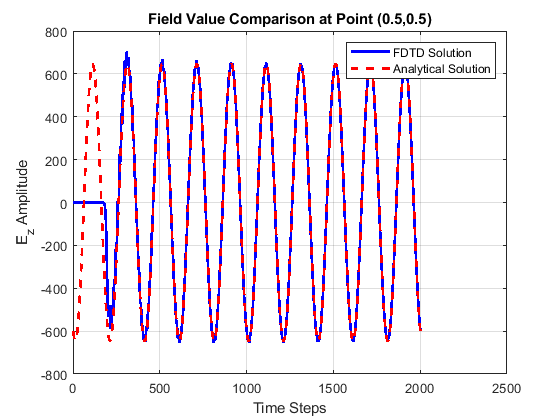
\includegraphics[width=0.23\textwidth]{figure/1a.png}
    }
    \hfill
    \subfloat[]{
        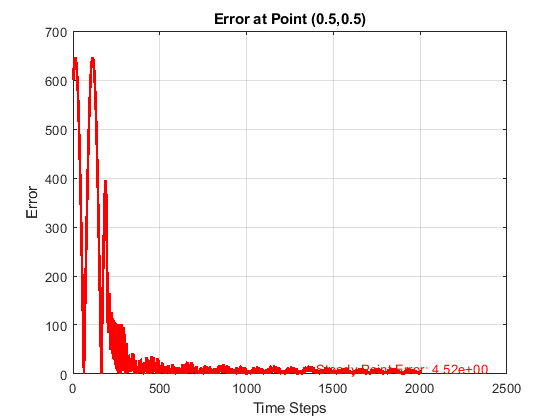
\includegraphics[width=0.23\textwidth]{figure/1b.png}
    }
    \caption{\small\textit{Comparison of FDTD and analytical solutions where $\Delta x = 0.005m$: (a) $E_z$ field values over time at (0.5m, 0.5m), (b) Error between FDTD and analytical solutions}}
    \label{fig:comparison}
\end{figure}

To reduce the computational cost, we in crease the grid size to $\Delta x = \Delta y = 0.01m$, and the error is around 1.5\% of the magnitude of the field, Fig. 2a,
which is still acceptable, and the simulation could be done within 30s on a single core CPU. When the grid size is further increased to 
$\Delta x = \Delta y = 0.02m$, the error is around 3\% of the magnitude of the field, Fig. 2b, so we stick to the grid size of $\Delta x = \Delta y = 0.01m$ for 
the following simulations.
\begin{figure}[htbp]
    \centering
    \subfloat[] {
        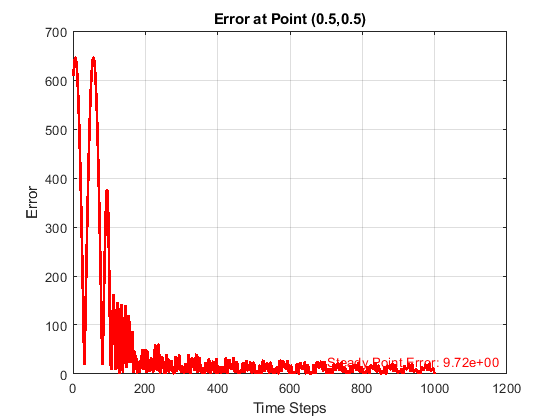
\includegraphics[width=0.23\textwidth]{figure/2a.png}
    }
    \hfill
    \subfloat[] {
        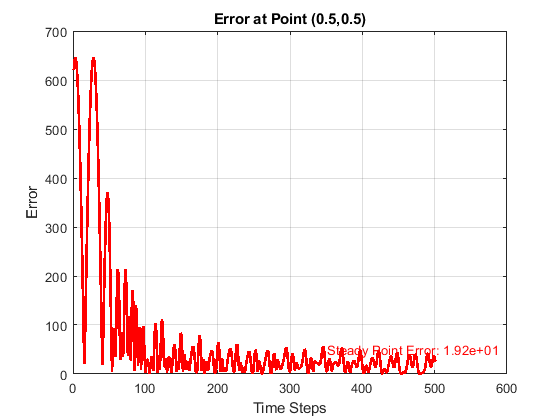
\includegraphics[width=0.23\textwidth]{figure/2b.png}
    }
    \caption{\small\textit{Comparison of FDTD and analytical solutions for different grid sizes: (a) $\Delta x = 0.01m$, (b) $\Delta x = 0.02m$}}
    \label{fig:grid_comparison}
\end{figure}

\subsection{PML Effectiveness}
To evaluate the effectiveness of the PML boundary conditions, we calculate the reflection coefficient at 
\begin{equation}
R = \left| \frac{\max(|E_z|_\text{near})}{\max(|E_z|_\text{inside})} - 1 \right|
\end{equation}

where $E_z|_\text{near}$ is the electric field measured at a point near the PML boundary, and $E_z|_\text{inside}$ 
at different observation points near the boundary. A smaller reflection coefficient indicates better PML performance. We conducted systematic tests varying both the polynomial order ($m$) and PML thickness to optimize performance, with results summarized in Table I.

\begin{table}[htbp]
\centering
\caption{PML Reflection Coefficients for Different Parameters}
\label{tab:pml_performance}
\begin{tabular}{|c|c|c|}
\hline
\textbf{Parameter} & \textbf{Value} & \textbf{Reflection Coefficient} \\
\hline
\multirow{4}{*}{$m$(while L = $\lambda$)} & 2 & $2.63 \times 10^{-2}$ \\
& 3 & $6.40 \times 10^{-2}$ \\
& 4 & $7.83 \times 10^{-2}$ \\
& 5 & $6.12 \times 10^{-2}$ \\
\hline
\multirow{3}{*}{L(while $m$=2)} & $0.2\lambda$ & $4.78 \times 10^{-2}$ \\
& $0.5\lambda$ & $1.53 \times 10^{-2}$ \\
& $1.0\lambda$ & $2.63 \times 10^{-2}$ \\
& $1.5\lambda$ & $8.05 \times 10^{-2}$ \\
\hline
\end{tabular}
\end{table}


Based on these results, a better configuration was determined to be a polynomial order $m=2$ with PML thickness of $0.5\lambda$, 
yielding the lowest reflection coefficient of $1.53 \times 10^{-2}$. This configuration was adopted for all subsequent simulations.
Fig. 3 shows the $E_z$ field distribution after the simulation has reached steady state, with the optimized PML configuration. The PML region is highlighted 
by the red dashed lines.

\begin{figure}[htbp]
    \centering
    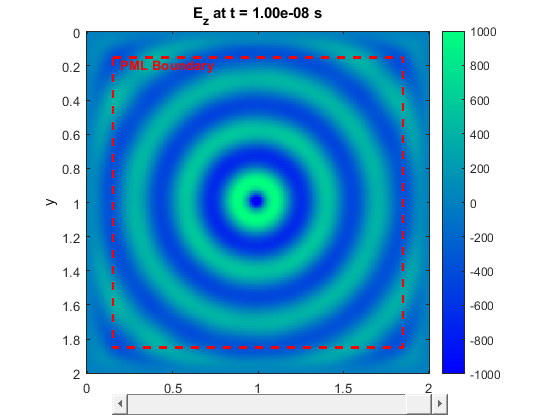
\includegraphics[width=0.35\textwidth]{figure/3.png}
    \caption{\small\textit{Steady-state $E_z$ field distribution showing effective wave absorption by the optimized PML. The red dashed lines indicate the PML boundaries.}}
    \label{fig:pml_effectiveness}
\end{figure}

\subsection{Single Slot Conductive Sheet and Double Slot Conductive Sheet}
To evaluate the FDTD-PML method in more complex scenarios, we introduced perfectly conducting sheets with apertures. 
For perfectly conducting sheets, we enforce the boundary condition $E_z = 0$ along the sheet surfaces, 
which follows from the requirement that the tangential electric field must vanish at the surface of a perfect electrical conductor (PEC).  

First, we simulated a single-slot conductive sheet positioned at x=0.5m. The slot was centered along the y-axis with a width of 0.1m. Figure 4 shows the $E_z$ field distribution at different time steps as waves interact with the sheet.

\begin{figure}[htbp]
    \centering
    \subfloat[]{
        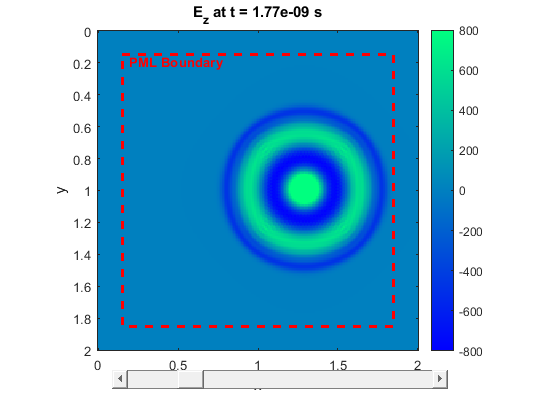
\includegraphics[width=0.23\textwidth]{figure/4a.png}
    }
    \hfill
    \subfloat[]{
        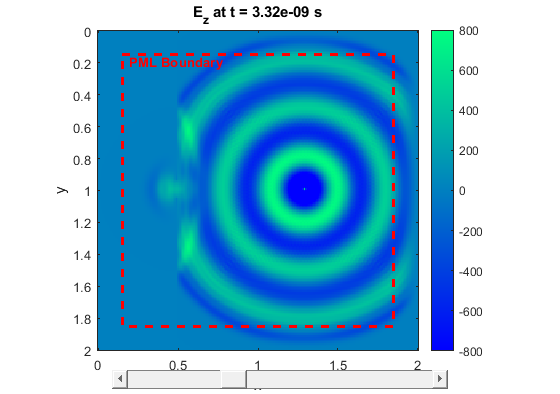
\includegraphics[width=0.23\textwidth]{figure/4b.png}
    }
    \hfill
    \subfloat[]{
        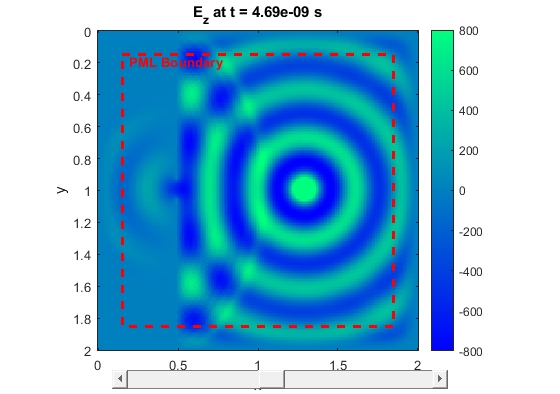
\includegraphics[width=0.23\textwidth]{figure/4c.png}
    }
    \hfill
    \subfloat[]{
        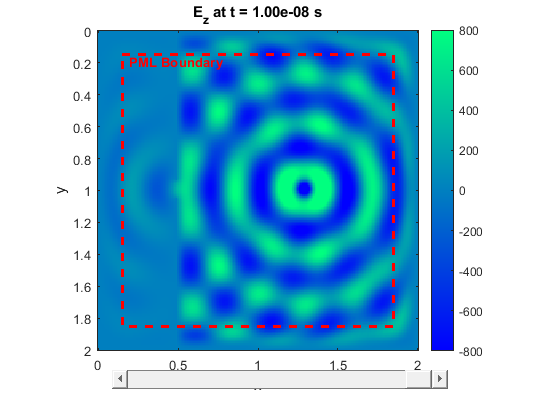
\includegraphics[width=0.23\textwidth]{figure/4d.png}
    }
    \caption{\small\textit{Evolution of $E_z$ field distribution as waves interact with a single-slot conductive sheet. }}
    \label{fig:single_slot}
\end{figure}

Subsequently, we implemented a double-slot configuration to examine more complex diffraction patterns. 
The two slots, each 0.1m wide, were positioned symmetrically at y=0.5m and y=1.5m. Figure 5 shows the $E_z$ field distribution at different time steps as waves interact with the sheet.
\begin{figure}[htbp]
    \centering
    \subfloat[]{
        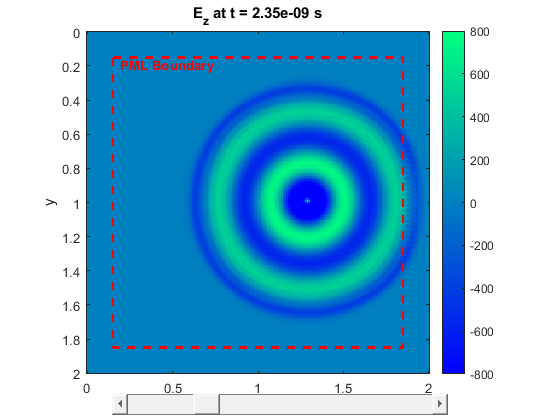
\includegraphics[width=0.23\textwidth]{figure/5a.png}
    }
    \hfill
    \subfloat[]{
        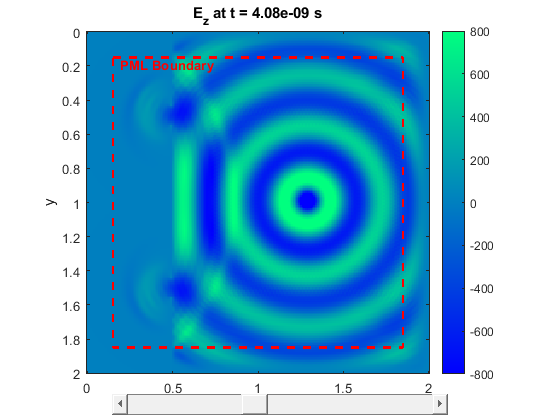
\includegraphics[width=0.23\textwidth]{figure/5b.png}
    }
    \hfill
    \subfloat[]{
        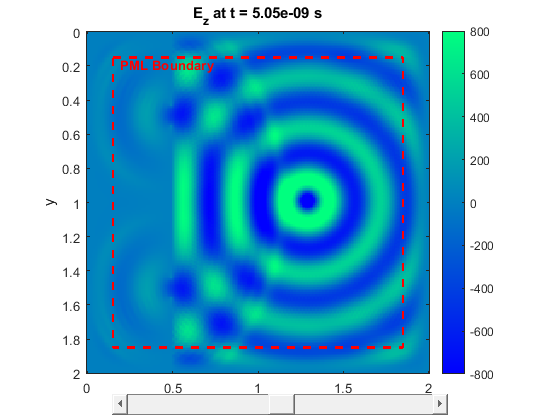
\includegraphics[width=0.23\textwidth]{figure/5c.png}
    }
    \hfill
    \subfloat[]{
        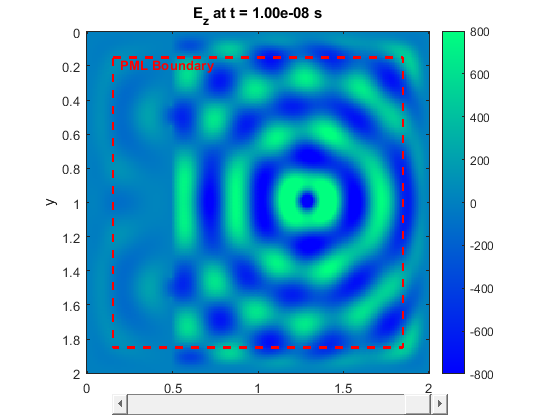
\includegraphics[width=0.23\textwidth]{figure/5d.png}
    }
    \caption{\small\textit{Evolution of $E_z$ field distribution as waves interact with a double-slot conductive sheet. }}
    \label{fig:double_slot}
\end{figure}

\section{Conclusion}
In this paper, we presented an FDTD implementation for analyzing the radiation characteristics of an infinite harmonic current line.
The Yee grid scheme was employed to discretize Maxwell's equations, 



\bibliographystyle{IEEEtran}
\begin{thebibliography}{9}

\bibitem{berenger1994perfectly}
J.-P. Berenger, "A perfectly matched layer for the absorption of electromagnetic waves," \emph{J. Comput. Phys.}, vol. 114, no. 2, pp. 185-200, 1994.

\bibitem{jin2011theory}
J.-M. Jin, \emph{Theory and Computation of Electromagnetic Fields}. Wiley, 2011.

\bibitem{yee1966numerical}
K. S. Yee, "Numerical solution of initial boundary value problems involving Maxwell's equations in isotropic media," \emph{IEEE Trans. Antennas Propag.}, vol. 14, no. 3, pp. 302-307, 1966.

\bibitem{jin2015theory}
J.-M. Jin, \emph{Theory and Computation of Electromagnetic Fields}. Wiley, 2015.
\end{thebibliography}

\end{document}